% STRATA: four-page version for work-in-progress and student-research tracks
% (IEEE conference format, 10 pt; 150-word abstract, at most six keywords).
% Build:  pdflatex short && bibtex short && pdflatex short && pdflatex short
% Numbers and table bodies are generated (../manuscript/tools/make_numbers.py).
%
% Double-blind review: uncomment the next line.
%\def\anonymous{1}
\documentclass[conference,10pt]{IEEEtran}
\usepackage{cite}
\usepackage{amsmath,amssymb,amsfonts}
\usepackage{graphicx}
\usepackage{textcomp}
\usepackage{url}

% generated by manuscript/tools/make_numbers.py from 20261013-143828-paper; do not edit
\newcommand{\AMFaster}{8}
\newcommand{\AMHi}{34.8}
\newcommand{\AMLo}{14.6}
\newcommand{\AllocHi}{99.9}
\newcommand{\AllocLo}{98.7}
\newcommand{\ArenaAbsMax}{10.7}
\newcommand{\ArenaFaster}{0}
\newcommand{\ArenaHi}{$+$10.7}
\newcommand{\ArenaLo}{$-$10.6}
\newcommand{\ArenaNE}{6}
\newcommand{\ArenaSlower}{2}
\newcommand{\BeforeHi}{33.8}
\newcommand{\BeforeLo}{11.4}
\newcommand{\BoundedDecls}{719\,833}
\newcommand{\BoundedLongest}{47}
\newcommand{\BoundedSamePeak}{True}
\newcommand{\BoundedTraces}{15}
\newcommand{\BytesHi}{36}
\newcommand{\BytesLo}{27}
\newcommand{\ChibiArenaFaster}{3}
\newcommand{\ChibiArenaHi}{$+$4.3}
\newcommand{\ChibiArenaLo}{$-$3.1}
\newcommand{\ChibiArenaSlower}{0}
\newcommand{\ChibiIdentArena}{158}
\newcommand{\ChibiIdentStrata}{158}
\newcommand{\ChibiRounds}{21}
\newcommand{\ChibiRssMedian}{0.18}
\newcommand{\ChibiStrataFaster}{0}
\newcommand{\ChibiStrataHi}{$+$2.2}
\newcommand{\ChibiStrataLo}{$-$3.7}
\newcommand{\ChibiStrataSlower}{1}
\newcommand{\ChibiUnitsAll}{170}
\newcommand{\ChibiUnitsOK}{158}
\newcommand{\DeclHi}{66}
\newcommand{\DeclLo}{56}
\newcommand{\DetCompared}{624}
\newcommand{\EmbBoundedPass}{5}
\newcommand{\EmbCode}{2\,715}
\newcommand{\EmbPass}{5}
\newcommand{\EmbStack}{492}
\newcommand{\EnvCPU}{Intel Core Ultra 7 258V}
\newcommand{\EnvCommit}{36f9f6c}
\newcommand{\EnvCompiler}{g++ 11.4.0}
\newcommand{\EnvKernel}{Linux 6.18.33.2-microsoft-standard-WSL2}
\newcommand{\ExhOps}{725\,594\,112}
\newcommand{\ExhRefusals}{130\,361\,632}
\newcommand{\ExhSeq}{80\,621\,568}
\newcommand{\ExitHi}{82}
\newcommand{\ExitLo}{71}
\newcommand{\FloodBoundedRatio}{2.5}
\newcommand{\FloodBoundedRefused}{32\,704}
\newcommand{\FloodCol}{1954}
\newcommand{\FloodExp}{1.96}
\newcommand{\FloodKeyedRatio}{1.2}
\newcommand{\FloodLookCol}{1684}
\newcommand{\FloodN}{32\,768}
\newcommand{\FloodOrd}{6.5}
\newcommand{\FloodRatio}{300}
\newcommand{\FuzzBefore}{9.8}
\newcommand{\FuzzFinal}{2.5}
\newcommand{\HeaderLines}{676}
\newcommand{\HeapLowerArena}{2}
\newcommand{\HeapMetisHi}{76}
\newcommand{\HeapMetisLo}{23}
\newcommand{\HeapMetisMed}{58}
\newcommand{\HeapSameArena}{6}
\newcommand{\IqrMedian}{16}
\newcommand{\KeyedHi}{32.2}
\newcommand{\KeyedLo}{20.2}
\newcommand{\LookHi}{$+$4.9}
\newcommand{\LookLo}{$-$20.3}
\newcommand{\MetisFaster}{8}
\newcommand{\MetisHi}{36.7}
\newcommand{\MetisLo}{15.9}
\newcommand{\MetisNE}{0}
\newcommand{\MetisRefused}{149}
\newcommand{\MetisRefusedOf}{400}
\newcommand{\MetisSlower}{0}
\newcommand{\MinBufHi}{156.5}
\newcommand{\MinBufLo}{15.8}
\newcommand{\Mutants}{9}
\newcommand{\NPairs}{104}
\newcommand{\NPairsAll}{195}
\newcommand{\NTables}{13}
\newcommand{\NTracesAll}{15}
\newcommand{\NoShrinkFaster}{2}
\newcommand{\NoShrinkHi}{$+$2.9}
\newcommand{\NoShrinkLo}{$-$4.9}
\newcommand{\NoShrinkSlower}{1}
\newcommand{\PackSaveHi}{9.0}
\newcommand{\PackSaveLo}{5.5}
\newcommand{\ProbeCells}{168}
\newcommand{\ProbeConfigs}{24}
\newcommand{\ProbeFiveTwelveBound}{$1.1\!\times\!10^{-7}$}
\newcommand{\ProbeFiveTwelveSeen}{0}
\newcommand{\ProbeHalfBound}{$1.0\!\times\!10^{-10}$}
\newcommand{\ProbeSamples}{10\,000\,000}
\newcommand{\ProbeSixtyFour}{0.77}
\newcommand{\ProbeTotal}{240\,000\,000}
\newcommand{\ProbeTwoFiftySix}{$2.0\!\times\!10^{-7}$}
\newcommand{\RawFaster}{0}
\newcommand{\RawHi}{$+$9.9}
\newcommand{\RawLo}{$-$1.6}
\newcommand{\RawSlower}{2}
\newcommand{\Rounds}{31}
\newcommand{\RunName}{20261013-143828-paper}
\newcommand{\SaveHi}{17.9}
\newcommand{\SaveLo}{16.4}
\newcommand{\SparseBufHi}{27}
\newcommand{\SparseBufLo}{18}
\newcommand{\SparseFaster}{6}
\newcommand{\SparseHi}{$-$4.5}
\newcommand{\SparseLo}{$-$12.9}
\newcommand{\SparseSlower}{0}
\newcommand{\SweepBestSave}{65}
\newcommand{\SynBadPairs}{1}
\newcommand{\SynCount}{9}
\newcommand{\SynFasterArena}{6}
\newcommand{\SynSlowerArena}{1}
\newcommand{\TotalDecls}{455\,122}
\newcommand{\TotalEvents}{1\,667\,499}
\newcommand{\UnitChecks}{2\,732\,358}
\newcommand{\UnitOnlySixteen}{23}
\newcommand{\UnitsTotal}{169}

\newcommand{\authorfill}[1]{\textbf{[AUTHOR: #1]}}
\makeatletter
\newcommand{\tabinput}[1]{\@@input #1.tex }
\makeatother
\newcommand{\st}{STRATA}
\newcommand{\code}[1]{\texttt{#1}}

\begin{document}

\title{Bounded Memory and Bounded Work for Scoped Symbol Tables: Work in Progress}

\ifdefined\anonymous
\author{\IEEEauthorblockN{Anonymous Author(s)}\IEEEauthorblockA{Submission for double-blind review}}
\else
\author{\IEEEauthorblockN{Shubhi Singh, Adhyan Jain, Akshith Venkatataramana, and Arjuman}
\IEEEauthorblockA{School of Computer Science and Engineering\\
Vellore Institute of Technology, Vellore, Tamil Nadu, India\\
\authorfill{confirm affiliations; add e-mail addresses}}}
\fi

\maketitle

\begin{abstract}
A compiler that runs inside a fixed memory budget needs a symbol table that is bounded in advance, fails in a defined way, and cannot be slowed down by hostile identifiers. We study a scoped symbol table that keeps its index, interned names and an undo stack in one caller-supplied buffer and leaves its state unchanged when an operation is refused. On symbol-table events logged by a C compiler for eight projects it needs a buffer \SaveLo\ to \SaveHi\ percent smaller than a conventional single-buffer table, with replay time within \ArenaAbsMax\ percent and no established difference on most traces. Because declarations are removed in reverse order of creation, the table always equals a freshly built one, which lets us bound how often a limit on index probes refuses an honest name. Identifiers that collide for every hash seed slow declarations \FloodRatio-fold; a keyed hash removes the effect.
\end{abstract}

\begin{IEEEkeywords}
compilers, embedded software, hash tables, linear probing, memory management, symbol tables
\end{IEEEkeywords}

\section{Problem}
A scoped symbol table maps identifiers to declarations and forgets a block's declarations when the block ends. The textbook implementation is a hash table with an undo stack~\cite{appel1998}; LLVM's \code{ScopedHashTable}~\cite{llvmsht} and the Tiny C Compiler~\cite{tcc} follow it. These tables allocate per symbol, leave their state undefined when an allocation fails, and use unkeyed hashes. For a compiler front end that must run in tens of kilobytes on source text it cannot trust, we ask for more: (R1) all state in one fixed buffer; (R2) an operation that does not fit is refused and changes nothing; (R3) a constant bound on the index slots one call examines; (R4) a negligible chance that this bound refuses an honest name. This paper reports what meeting R1 to R4 costs. The algorithm is the textbook one; what we contribute is the construction around it, two properties that follow from it, and a measurement against a baseline that shares its constraints.

\section{Design}
\begin{figure}[t!]
\centering
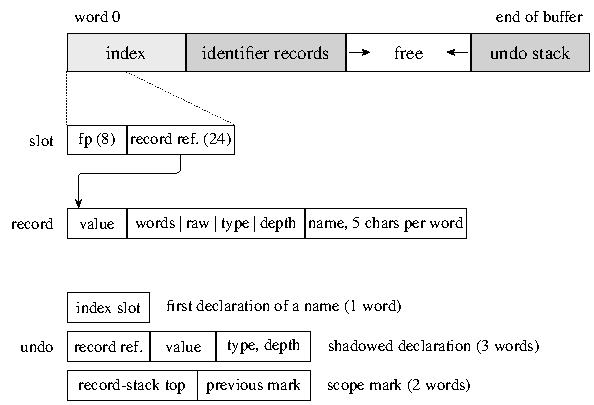
\includegraphics[width=0.94\columnwidth]{figures/fig_layout.pdf}
\caption{One buffer of 32-bit words: index, identifier records and undo stack.}
\label{fig:layout}
\end{figure}

\st\ keeps everything in one array of 32-bit words (Fig.~\ref{fig:layout}). The index is a linear-probing table of slots holding an 8-bit fingerprint and a record reference, at most three quarters full. There is one record per distinct visible name; it holds the value of the \emph{innermost} declaration, so a lookup ends in the record it finds whatever the shadowing depth. Names made of identifier characters are packed five to a word. A declaration of a new name pushes one undo word, its index slot; a declaration that hides an outer one pushes three words, what it overwrote.

\emph{Refusal.} Every operation searches, reserves, and only then writes, so a refusal (buffer full, nesting limit, invalid name, probe limit) leaves every word unchanged.

\emph{Scope exit without tombstones.} In linear probing without displacement, the slots between a key's home and its position were occupied by older keys when it was inserted. The newest key therefore lies on no other key's path and can be removed by emptying its slot. Scope exit removes declarations newest first, so it writes no tombstone and moves no key.

\emph{Canonical state.} It follows by induction that after any sequence of operations the table is, word for word, a fresh table into which only the live declarations were made. The table does not age, and at every moment its index is that of insertion-only linear probing.

\emph{Bounded mode.} With an index of fixed size and a limit of $L$ probes, a new name is inserted only if an empty slot lies among the first $L$ slots of its path, and is refused otherwise; lookups stop after $L$ slots. Dictionaries that bound probes by moving keys, such as cuckoo~\cite{pagh2004} and hopscotch hashing~\cite{herlihy2008}, would break the removal rule above. Because the index is an insertion-only table, the standard interval argument~\cite{thorup2015} applies: for $n$ names with independent uniform home slots in $m$ slots, $\alpha = n/m$ and $\rho = \alpha e^{1-\alpha}$,
\begin{equation}
\Pr[\text{a new name is refused}] \;\le\; \rho^{L}/(1-\rho).
\label{eq:bound}
\end{equation}
An optional keyed hash, HalfSipHash with one and three rounds~\cite{aumasson2012,linuxsiphash}, makes the assumption hold for names chosen by someone who does not know the key.

\section{Evaluation}
\emph{Method.} We logged the symbol-table calls of the Tiny C Compiler~\cite{tcc} on eight open-source C projects (\TotalEvents\ events) and replay them on \NTables\ tables, checking every result against an independent reference model. The main baseline is a conventional chained table in one buffer with the same refusal discipline, written to be as strong as we could make it; METIS-X~\cite{metis} is the multi-allocation predecessor of this work. Timing uses \Rounds\ rounds in which every table replays each trace once in rotating order; we report the median per-round ratio with a 95 percent bootstrap interval. All measurements are from one laptop.

\begin{table*}[t!]
\caption{Smallest fixed buffer (KiB) and replay time of \st\ relative to the conventional single-buffer table and to METIS-X (percent, 95 percent interval; negative is faster).}
\label{tab:short}
\centering
\setlength{\tabcolsep}{6pt}
\begin{tabular}{|l|r|r|r|l|l|}
\hline
Project & \st\ buffer & Conventional buffer & Saving (\%) & Time vs. conventional table & Time vs. METIS-X \\
\hline
\tabinput{tables/tab_short}
\end{tabular}
\end{table*}

\emph{Memory and time.} All tables agree with the reference model on every trace. Table~\ref{tab:short} gives the result: \st\ needs a fixed buffer \SaveLo\ to \SaveHi\ percent smaller than the conventional table, \BytesLo\ to \BytesHi\ bytes per live declaration. In time it is faster on \ArenaFaster\ traces, slower on \ArenaSlower, and not distinguishable on \ArenaNE. Against METIS-X it is faster on \MetisFaster\ of 8, but so is the conventional table (\AMLo\ to \AMHi\ percent): most of that gain comes from one allocation-free buffer, not from the compact layout.

\emph{A penalty that was an artifact.} An earlier version was \BeforeLo\ to \BeforeHi\ percent slower than the conventional table on every trace. Per-operation latencies placed the difference in declarations, and the cause was rebuild work: the index was rebuilt whenever the buffer grew, although it does not move; every rebuild hashed each name twice; and a new name walked its probe path twice. Removing these left memory and all results unchanged and the two tables within about ten percent of each other (Fig.~\ref{fig:time}).

\begin{figure}[t!]
\centering
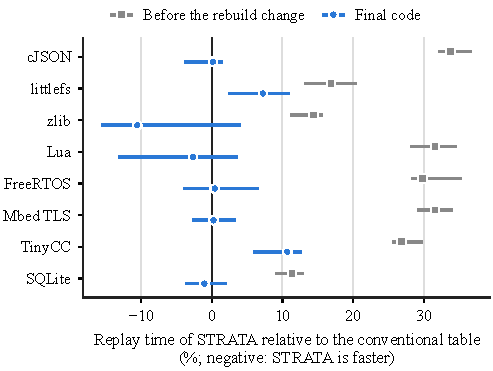
\includegraphics[width=0.94\columnwidth]{figures/fig_time.pdf}
\caption{Replay time of \st\ relative to the conventional table before and after the rebuild change (median of paired ratios, 95 percent interval).}
\label{fig:time}
\end{figure}

\emph{Inside a compiler.} With chibicc's variable scopes on \st, the generated assembly is identical on \ChibiIdentStrata\ of \ChibiUnitsOK\ translation units and whole-project compile time changes by between \ChibiStrataLo\ and \ChibiStrataHi\ percent: in a hosted compiler the table does not matter.

\begin{figure}[t!]
\centering
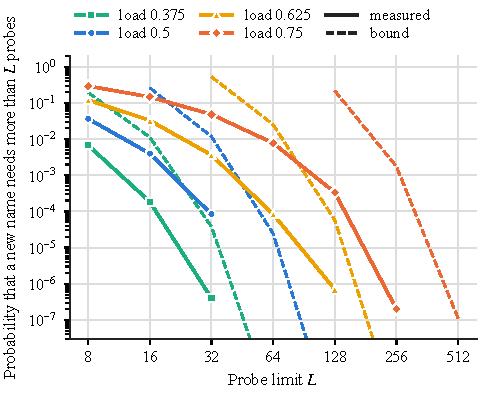
\includegraphics[width=0.94\columnwidth]{figures/fig_probe.pdf}
\caption{Probability that inserting a fresh name examines more than $L$ slots (keyed hash, 65\,536 slots, \ProbeSamples\ samples per load) and the bound \eqref{eq:bound}.}
\label{fig:probe}
\end{figure}

\emph{Hostile identifiers.} The default hash is a MurmurHash3-style mixer. Following Aumasson and Bernstein~\cite{aumasson2012}, we build \FloodN\ valid C identifiers that collide for every seed, restricting the construction to words that are packings of identifier characters. Declaring them takes \FloodCol\,ms against \FloodOrd\,ms for ordinary names of the same length, with quadratic growth. Under the keyed hash the ratio is \FloodKeyedRatio; the keyed hash costs \KeyedLo\ to \KeyedHi\ percent of replay time on the compiler traces.

\emph{The probe limit.} Replaying \BoundedTraces\ compiler traces in bounded mode, a limit of 64 refuses none of \BoundedDecls\ declarations. That observation does not generalize. Simulating insertions with the table's own hash (Fig.~\ref{fig:probe}), the bound was never exceeded in \ProbeCells\ configurations, and at the load limit of $3/4$, \ProbeSixtyFour\ percent of fresh names need more than 64 probes. The bound supports a limit of 512 (at most \ProbeFiveTwelveBound\ per declaration; none seen in \ProbeSamples\ samples).

\emph{Evidence for the guarantees.} \UnitChecks\ randomized differential checks under sanitizers; every sequence of nine operations over four names in eight small configurations (\ExhSeq\ sequences); \FuzzFinal\ million fuzzing executions of the final code; and a mutation check in which the fuzzer detects all \Mutants\ injected defects. On an emulated Cortex-M3 with 64\,KiB of memory and no heap, five traces replay with host-identical results in \EmbCode\ bytes of code.

\section{Limitations and Next Steps}
The measurements are replays on one machine; the microcontroller is emulated; the workloads are C only; the baselines other than METIS-X are our own; the two properties are argued, tested and enumerated but not machine-checked; the bound assumes an ideal hash; per-trace timing verdicts vary between runs; and the literature search was limited. The collision construction is a known technique. Next: a compiler that actually runs on the table on a physical device under a budget, a checked proof, and workloads from other languages.

\ifdefined\anonymous
\else
\section*{Acknowledgment}
The authors thank Bhuvaneswari~M. for guiding the project. The implementation, experiments, analysis and text were produced with the assistance of an artificial-intelligence coding assistant (Claude, Anthropic) at the direction of the first author. \authorfill{review, verify and adapt this statement to the venue's policy.} The artifact is public~\cite{strata}.
\fi

\bibliographystyle{IEEEtran}
\bibliography{references}

\end{document}
